





 Line $l$ is tangent to the circle at point $A$.  If point $C$ is the center of the circle and $m\angle ADC =30^\circ$, then what is the measure of $\angle ABD$?
\begin{center}
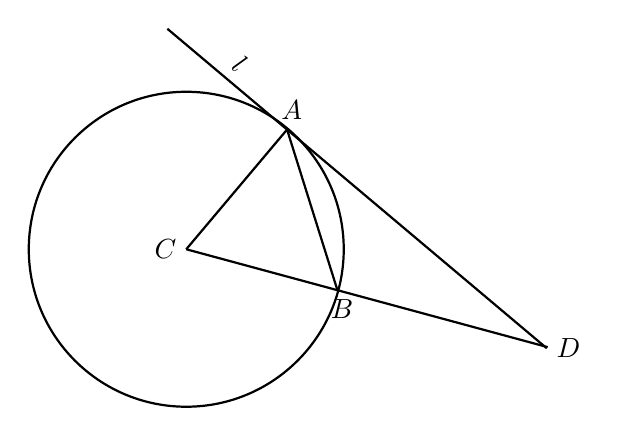
\begin{tikzpicture}
    \draw[thick] (0,0) circle (2cm);
    \draw[thick] (0,0)--(2*.64, 2*.76);
\draw (0,0) node [left] {$C$};
\draw (2*.64, 2*.76) node [above] {$\,\,A$};
\draw (2*.96, 2*-.26) node [below] {$\,\,B$};
\draw (2*.64+2.17*2*.76, 2*.76-2.17*2*.64) node [right] {$D$};
    \draw[thick] (0,0)--(4.78*.96, 4.78*-.26);
    \draw[thick] (2*.64, 2*.76)--(2*.96, 2*-.26);
    \draw[thick] (2*.64-2*.76, 2*.76+2*.64)--(2*.64, 2*.76)  node[midway, above, sloped]{$l$}; 
    \draw[thick] (2*.64+2.17*2*.76, 2*.76-2.17*2*.64)--(2*.64, 2*.76); 
               
        
\end{tikzpicture}
\end{center}



\ifsat
	\begin{enumerate}[label=\Alph*)]
		\item   $30^\circ$
		\item  $90^\circ$
		\item  $120^\circ$ %
		\item  $140^\circ$ 
	\end{enumerate}
\else
\fi

\ifacteven
	\begin{enumerate}[label=\textbf{\Alph*.},itemsep=\fill,align=left]
		\setcounter{enumii}{5}
		\item   $30^\circ$
		\item  $60^\circ$
		\item  $90^\circ$
		\addtocounter{enumii}{1}
		\item  $120^\circ$ %
		\item  $140^\circ$ 
	\end{enumerate}
\else
\fi

\ifactodd
	\begin{enumerate}[label=\textbf{\Alph*.},itemsep=\fill,align=left]
		\item   $30^\circ$
		\item  $60^\circ$
		\item  $90^\circ$
		\item  $120^\circ$ %
		\item  $140^\circ$ 
	\end{enumerate}
\else
\fi

\ifgridin
  $120^\circ$ %
		
\else
\fi

